\chapter{Related work}

\section{Introduction}

\section{Technological foundations}

\section{Existing solutions}

Before starting with our own app, we felt that a way of gathering... 
was looking into already existing solutions in the market to see 
what we liked or not...??? 

This section reviews 3 applications that propose similar solutions to what 
we wanted to do. The solutions analysed are: Tomplay, Oktav and Newzik.

\subsection{Tomplay}

\todo[inline]{Review why citations are not appearing.}

Tomplay~\cite{tomplay} is a mobile and desktop app.

\begin{figure}[H]
	\centering
	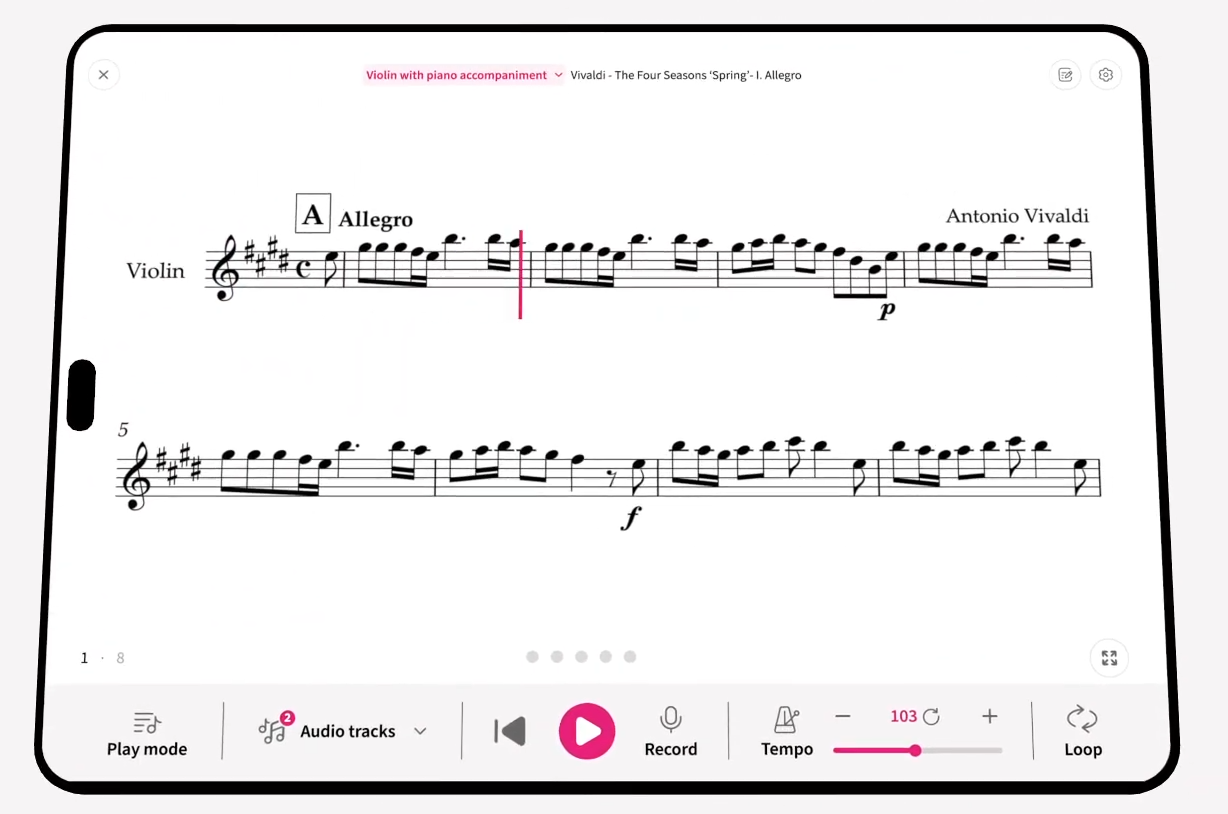
\includegraphics[width=0.6\textwidth]{Images/tomplay.png}
	\caption{Tomplay user interface.}
	\label{fig:tomplay}
\end{figure}

Its main features are:
\begin{itemize}
	\item \textbf{Digital sheet music}: Automatically scrolls in sync with the music.
	\item \textbf{Note by note practice}: The score advances only when you play the right note.
	\item \textbf{Adjust the tempo}: Slow down or speed up the music tempo.
	\item \textbf{Record yourself}: Record and listen back to your performance.
	\item \textbf{Annotate}: Add your own annotations to the music sheet.
	\item \textbf{Big music sheet catalogue}: Over 100,000 scores with professional audio accompaniments.
\end{itemize}

However, it presents some limitations:
\begin{itemize}
	\item Paid subscription
	\item 
	\item 
\end{itemize}

\todo[inline]{Add some more limitations.}


\subsection{OKTAV}

OKTAV~\cite{oktav} is a web app.

\begin{figure}[H]
	\centering
	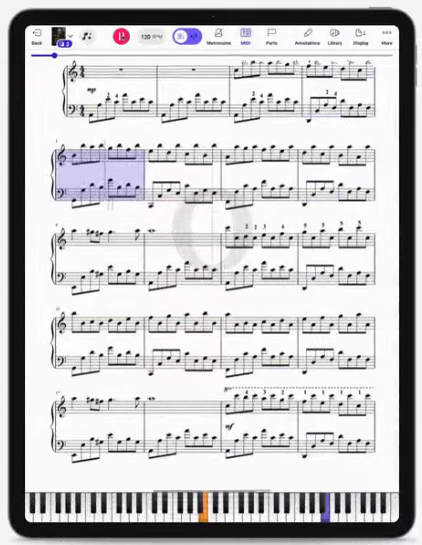
\includegraphics[width=0.4\textwidth]{Images/oktav.png}
	\caption{Oktav user interface.}
	\label{fig:oktav}
\end{figure}

Its main features are:
\begin{itemize}
	\item \textbf{Autoscroll}: Play without the need to turn pages and adjust tempo.
	\item \textbf{Annotate}: Ability to add fingerings, notes or highlight sections.
	\item \textbf{Play-along}: listen and play along to sheet music based on MIDI.
	\item \textbf{Digital piano}: See how to play a music sheet on a visual keyboard shown along the music sheet. 
\end{itemize}

Its limitations are:
\begin{itemize}
	\item Paid subscription
	\item Only for piano, violin and cello
	\item 
\end{itemize}

\subsection{Newzik}

Newzik~\cite{newzik}
is a web and mobile app.

\begin{figure}[H]
	\centering
	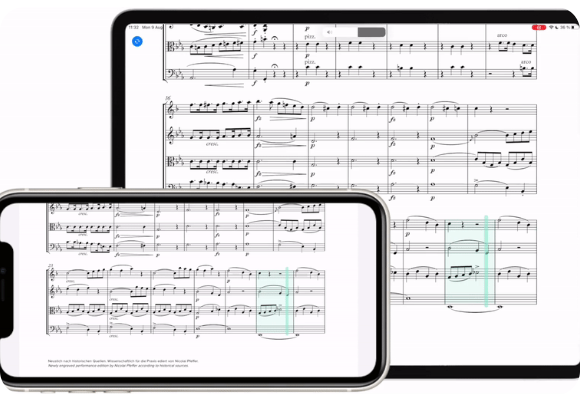
\includegraphics[width=0.6\textwidth]{Images/newzik.png}
	\caption{Newzik user interface.}
	\label{fig:newzik}
\end{figure}

Its main features are:
\begin{itemize}
	\item \textbf{Organization}: Centralize your digital sheet music (PDFs, scans, sets).
	\item \textbf{Play \& listen}: Listen to your sheet music with an AI that reads it for you.
	\item \textbf{Annotate \& turn pages}: Highlight, add fingerings and markers, and turn pages hands-free using facial movements (or a Bluetooth pedal).
\end{itemize}

Its limitations are:
\begin{itemize}
	\item Paid subscription
	\item Mobile app is only available for iOS
	\item No real-time tracking, you need to use gestures or a pedal to turn pages
\end{itemize}

\section{Comparison with the proposed solution}

Table~\ref{tab:existing-solutions} summarises the main characteristics of the solutions reviewed and our app.

\todo[inline]{Fill in the table below}

\begin{table}[H]
	\centering
	\begin{tabularx}{\textwidth}{l Y Y Y Y}
		\toprule
		\textbf{Feature} & \textbf{Tomplay} & \textbf{Oktav} & \textbf{Newzik} & \textbf{AtrilMatic} \\
		\midrule
		Platform			& Mobile and desktop	& Web 			& Web and iOS	& Web \\
		Price				& Paid 					& Paid 			& Paid 			& Free \\
		Score format		& Paid 					& Paid 			& Paid 			& PDF, MusicXML, XML \\
		Real-time tracking	& Paid 					& Paid 			& Paid 			& Yes \\
		Automatic page turn	& Paid 					& Paid 			& No 			& Yes \\
		Performance stats	& Paid 					& Paid 			& Paid 			& Not for now \\
		\bottomrule
	\end{tabularx}
	\caption{Comparison of existing solutions.}
	\label{tab:existing-solutions}
\end{table}